% Kap. 1 -- Neuaufbau 2026-11-05, Stil "luftig" 2026-11-06 (Backup: ../elektronik-1_backup_2026-11-05)
\section{Grundlagen}\label{sec:grundlagen}

\subsection{DC und AC getrennt}

{\renewcommand{\arraystretch}{1.5}
\begin{tabularx}{\columnwidth}{@{}l l X@{}}
	\toprule
	\textbf{Bauteil}   & \textbf{DC (Arbeitspunkt)} & \textbf{AC (Signal)} \\ \midrule
	DC-Spannungsquelle & wirkt                      & Kurzschluss \\
	DC-Stromquelle     & wirkt                      & offen \\
	Kondensator $C$    & offen                      & Kurzschluss, wenn $X_C = \dfrac{1}{2\pi f C} \ll R$ im Pfad \\
	Spule $L$          & Kurzschluss                & offen \\
	Nichtlinear (Diode, BJT) & Kennlinie            & Kleinsignal-ESB ($r$ im AP) \\ \bottomrule
\end{tabularx}}

\begin{rezept}{Rezept: Schaltungsanalyse}
	\begin{steps}
		\item \textbf{DC}: Arbeitspunkt, DC-Spannung in jedem Knoten
		\item \textbf{AC}: Signalpfad nach der Tabelle oben, Verstärkung $A_k$ jeder Quelle
		\item \textbf{Störquellen} (z.B. Rippel auf $V_{\rm DD}$): eigener AC-Pfad wie ein Eingang
		\item \textbf{Kontrolle}: Ausgang innerhalb der Speisung? Sonst Sättigung
	\end{steps}
	$$ v_{\rm out}(t) = V_{\rm out,DC} + \sum_k A_k\,\hat v_k \sin(2\pi f_k t) $$
\end{rezept}

\warn{\textit{La Superposition vale solo nel tratto lineare: con l'uscita al rail (Sättigung) non vale più.}}
\warn{\textit{Anche AGND, VCOM, $V_{\rm ref}$ e $V_{\rm DD}$ sono sorgenti: ognuna ha il suo termine.}}

\subsection{Gross- und Kleinsignal}

\begin{minipage}[t]{0.48\columnwidth}
	\textbf{Grosssignal} (Gerade durch Ursprung)
	$$ R = \frac{V_{\rm AP}}{I_{\rm AP}} $$
\end{minipage}
\hfill
\begin{minipage}[t]{0.48\columnwidth}
	\textbf{Kleinsignal} (Tangente im AP)
	$$ r = \frac{\diff V}{\diff I} \approx \frac{\Delta V}{\Delta I} $$
\end{minipage}

\subsection{Verstärker}

{\renewcommand{\arraystretch}{1.4}
\begin{tabular}{@{}l l@{\qquad}l l@{}}
	Spannung:   & $v_{\rm out} = A_v\, v_{\rm in}$ & Strom:      & $i_{\rm out} = A_i\, i_{\rm in}$ \\
	Transkond.: & $i_{\rm out} = g_m\, v_{\rm in}$ & Transimp.:  & $v_{\rm out} = R_m\, i_{\rm in}$
\end{tabular}}

\vspace{4pt}
\textbf{Kette realer Verstärker}: $R_{\rm out}$ und das nächste $R_{\rm in}$ bilden einen Spannungsteiler.

\begin{center}
	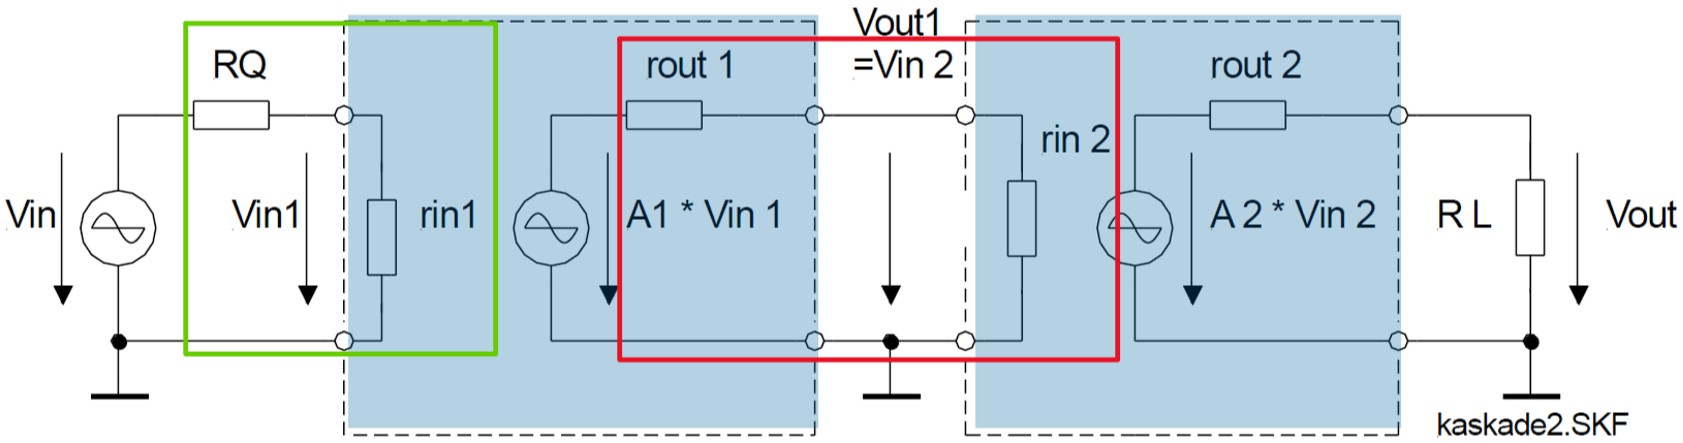
\includegraphics[width=0.8\columnwidth]{images/kopplungsfaktor.jpg}
\end{center}

$$ \boxed{ v_{\rm out} = v_{\rm in}\, k_1 A_1\, k_2 A_2\, k_L } $$
$$ k_1 = \frac{R_{\rm in1}}{R_{\rm in1}+R_Q} \qquad k_2 = \frac{R_{\rm in2}}{R_{\rm in2}+R_{\rm out1}} \qquad k_L = \frac{R_L}{R_L + R_{\rm out2}} $$

\textbf{Dezibel} (in Serie: dB addieren)
$$ A_{\rm dB} = 20 \log |A| \qquad\Longleftrightarrow\qquad A = 10^{A_{\rm dB}/20} $$
\begin{center}
\renewcommand{\arraystretch}{1.3}
\begin{tabular}{@{}l|cccccc@{}}
	$|A|$ & $0.5$ & $1/\sqrt2$ & $2$ & $10$ & $100$ & $1000$ \\ \hline
	dB    & $-6$  & $-3$       & $6$ & $20$ & $40$  & $60$
\end{tabular}
\end{center}

\subsection{Toleranzen und Worst-Case}\label{sec:worstcase}

\begin{rezept}{Rezept: Worst-Case mit Toleranz $\pm t$}
	\begin{steps}
		\item Resultat $f(R_1, R_2, \dots)$ \textbf{symbolisch} aufstellen
		\item Für jedes $R$ entscheiden: wird $f$ grösser, wenn $R$ grösser wird?
		\item $f_{\max}$: jedes $R$ an die günstige Grenze $R(1\pm t)$; \; $f_{\min}$: alle umgekehrt
	\end{steps}
	\vspace{2pt}
	{\renewcommand{\arraystretch}{1.4}
	\begin{tabularx}{\linewidth}{@{}l X@{}}
		$R$ nur im Zähler  & $R$ gross \textrightarrow\ $f$ gross \\
		$R$ nur im Nenner  & $R$ gross \textrightarrow\ $f$ klein \\
		$R$ in beiden      & umformen: \; $\dfrac{R_2}{R_1+R_2} = \dfrac{1}{1+R_1/R_2}$
	\end{tabularx}}
\end{rezept}

\textbf{Spannungsteiler}, Maximum:
$$ V_{\max} = V\, \frac{R_2(1+t)}{R_1(1-t) + R_2(1+t)} $$
\textbf{Faustregel}: bei Produkt oder Quotient addieren sich die relativen Toleranzen ($\frac{R_2}{R_1}$ mit je $\pm1\,\%$ \textrightarrow\ $\pm 2\,\%$).

\warn{\textit{Stesso valore nominale $\neq$ stesso valore reale: nel worst case ogni R va al suo estremo in modo indipendente (es. DAC, Kap.~4).}}
